\documentclass[12pt]{article}

\usepackage[utf8]{inputenc}


\usepackage{caption}
\usepackage{amsmath}
\usepackage{graphicx}
\usepackage{amssymb}
\usepackage{float}
\usepackage{multirow}
% set font size to 11pt


\setlength{\parskip}{\baselineskip}%
\setlength{\parindent}{0pt}%

\begin{document}

\title{Wave Transmission}
\author{lwp26}
\date{Feburary 2023}
\maketitle


\section{Introduction}

\subsection{Background}

Waves are a fundamental part of physics with many different applications,
in the efficient transmission of information and energy. 
In this report, we will be looking at the transmission of waves through a medium, 
and how the transmission of waves can be affected by the medium.


\subsection{Aims}
\begin{itemize}
    \item To create and observe the effect of combining waves travelling in opposite directions - 
    which produces standing waves.
    \item To measure the wavelength and velocity of microwaves in air by observing standing waves
    in a coaxial line.
    \item To measure the velocity of microwaves in some solid material (e.g. teflon, perspex and
    glass) from the change in travel time when the material is substituted for air, and to
    characterise the material by its refractive index, n.
    \item To build a microwave resonator, by making a section line with highly reflective ends. To
    plot and interpret the response versus frequency for resonators of two different lengths.
    \item To identify sources of error in the instruments and procedures used, and to suggest
    improvements.
\end{itemize}

\section{Results}

\begin{center}
    \captionof{table}{Measurements of wavelength and phase velocity of standing waves}
    \begin{tabular}{|c|c|c|c|c|c|}
    \hline
    Freq. & \multicolumn{2}{|c|}{Minima Positions} & N. Maximas &$\lambda$ & $u$ \\
    $f$/GHz & $P_1$/mm & $Q_1$/mm & $P_1$ to $Q_1$ & mm & mm/ns\\
    \hline 
    2.399	& 22	& 523	& 8	    & 125.25	& 300.475 \\
    3.000	& 59	& 452	& 8	    & 98.25	    & 294.75 \\
    3.600	& 30	& 488	& 11	& 83.27	    & 299.782 \\
    \hline
    \end{tabular}
\end{center}

\begin{center}
    \captionof{table}{Amplitude reflection coefficients measured with slotted line}
    \begin{tabular}{|c|c|c|c|c|c|c|}
    \hline
    $f$ & $P_2$ & $(P_2-P_1)$ & $Q_2$ & $(Q_2-Q_1)$ & Average Shift & $\Delta / \lambda$ \\
    GHz & mm & mm & mm & mm & $\Delta$ mm & - \\
    \hline 
    3.0 & 33 & 26 & 431 & 21 & 23.5 & 0.239185751 \\
    \hline
    \end{tabular}
\end{center}

\begin{center}
    \captionof{table}{Velocity of microwaves in different materials}
    \begin{tabular}{|c|c|c|c|c|c|}
    \hline
    Material & M /mm & d /mm & R /mm & R-M /mm & n \\
    \hline  
    \multirow{4}{*}{Perspex}& 49	& 30	& 60	& 11	& 1.37 \\
        	                & 52	& 60	& 64	& 12	& 1.20 \\
        	                & 52	& 90	& 70	& 18	& 1.20 \\
        	                & 52	& 120	& 71	& 19	& 1.16 \\
    \hline
    \multirow{4}{*}{Glass}	& 52	& 30	& 64	& 12	& 1.40 \\
        	                & 52	& 60	& 81	& 29	& 1.48 \\
        	                & 52	& 90	& 56	& 4	    & 1.04 \\
        	                & 52	& 120	& 69	& 17	& 1.14 \\
    \hline
    \multirow{4}{*}{Teflon}	& 52	& 30	& 60	& 8	    & 1.27 \\
                        	& 52	& 60	& 65	& 13	& 1.22 \\
                        	& 52	& 90	& 68	& 16	& 1.18 \\
                        	& 52	& 120	& 75	& 23	& 1.19 \\
    \hline
    \end{tabular}
\end{center}

\begin{figure}[h]
    \centering
    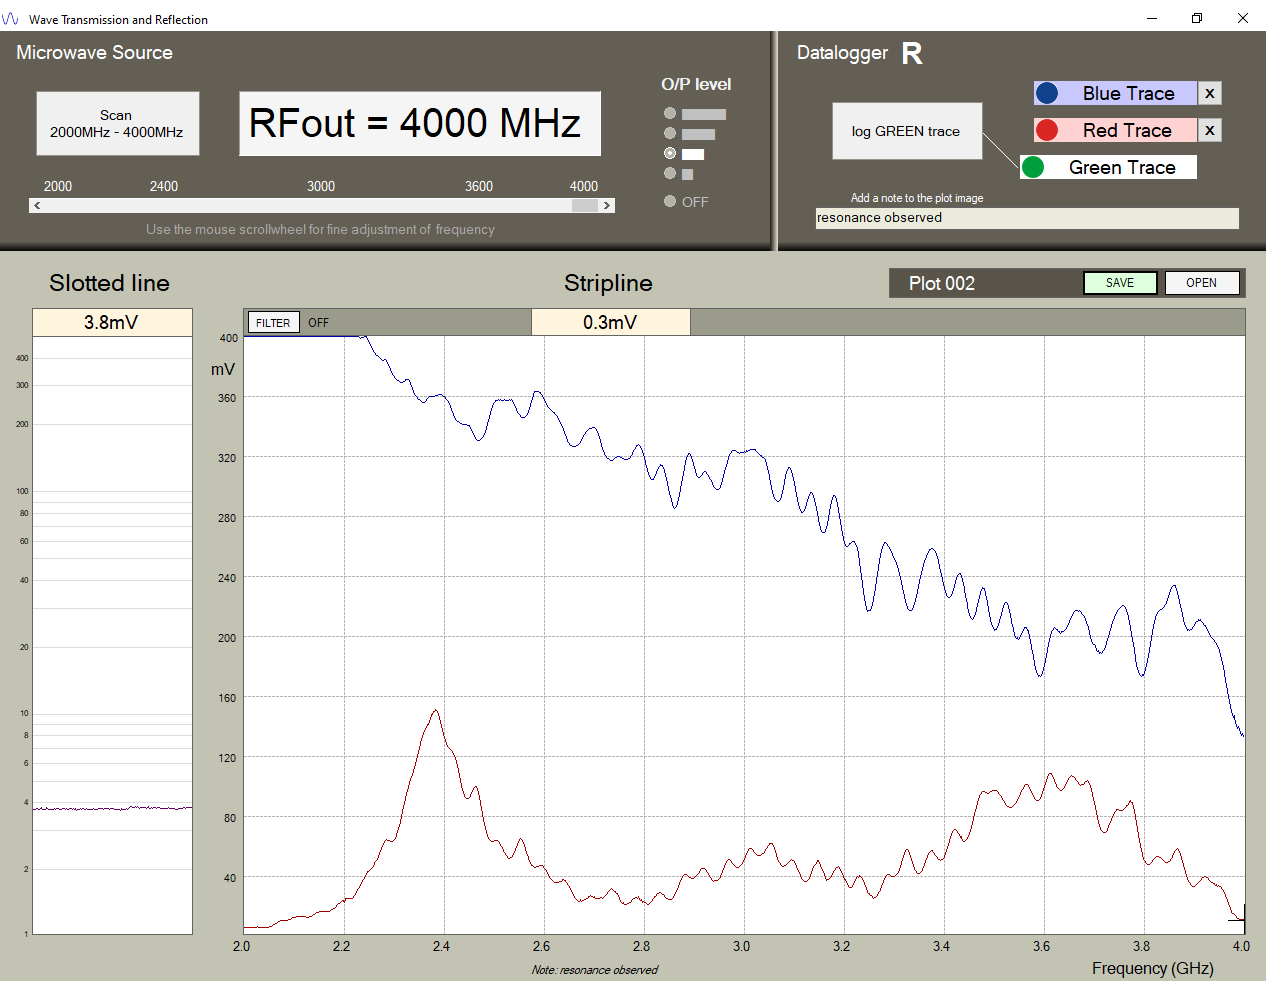
\includegraphics[width=1\textwidth]{Plot_2.png}
    \caption{Graph showing resonance}
    \label{fig:phase_space}
\end{figure}

\end{document}